% Created by tikzDevice version 0.12.3.1 on 2021-03-17 17:12:37
% !TEX encoding = UTF-8 Unicode
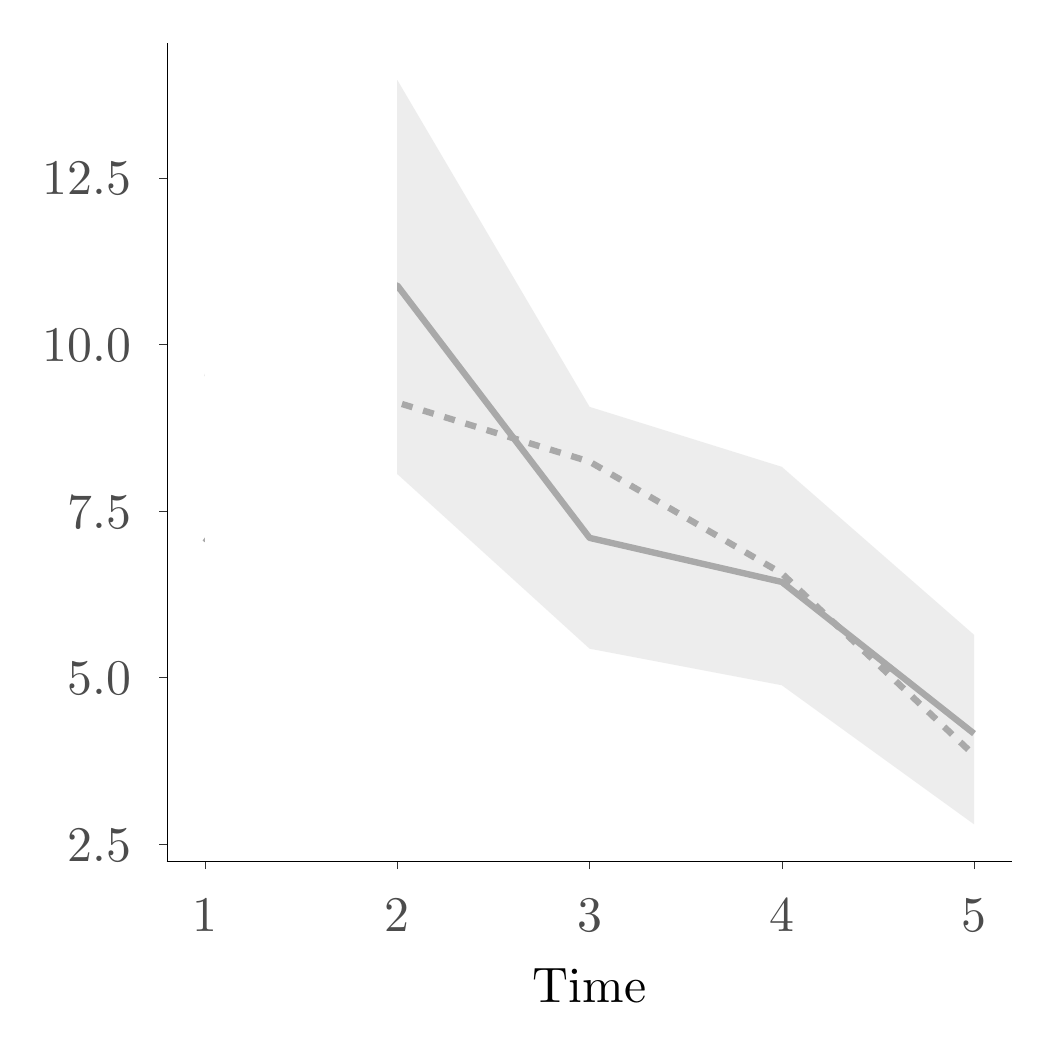
\begin{tikzpicture}[x=1pt,y=1pt]
\definecolor{fillColor}{RGB}{255,255,255}
\path[use as bounding box,fill=fillColor,fill opacity=0.00] (0,0) rectangle (361.35,361.35);
\begin{scope}
\path[clip] (  0.00,  0.00) rectangle (361.35,361.35);
\definecolor{drawColor}{RGB}{255,255,255}
\definecolor{fillColor}{RGB}{255,255,255}

\path[draw=drawColor,line width= 0.1pt,line join=round,line cap=round,fill=fillColor] (  0.00,  0.00) rectangle (361.35,361.35);
\end{scope}
\begin{scope}
\path[clip] ( 50.24, 60.04) rectangle (355.85,355.85);
\definecolor{fillColor}{RGB}{255,255,255}

\path[fill=fillColor] ( 50.24, 60.04) rectangle (355.85,355.85);
\definecolor{fillColor}{RGB}{169,169,169}

\path[fill=fillColor,fill opacity=0.20] ( 64.13,269.42) --
	(133.59,342.40) --
	(203.05,224.33) --
	(272.50,202.66) --
	(341.96,141.97) --
	(341.96, 73.49) --
	(272.50,123.73) --
	(203.05,136.94) --
	(133.59,200.03) --
	( 64.13, 96.43) --
	cycle;

\path[] ( 64.13,269.42) --
	(133.59,342.40) --
	(203.05,224.33) --
	(272.50,202.66) --
	(341.96,141.97);

\path[] (341.96, 73.49) --
	(272.50,123.73) --
	(203.05,136.94) --
	(133.59,200.03) --
	( 64.13, 96.43);
\definecolor{drawColor}{RGB}{169,169,169}

\path[draw=drawColor,line width= 2.3pt,line join=round] ( 64.13,175.32) --
	(133.59,268.15) --
	(203.05,176.98) --
	(272.50,161.06) --
	(341.96,106.26);

\path[draw=drawColor,line width= 2.3pt,dash pattern=on 4pt off 4pt ,line join=round] ( 64.13,236.56) --
	(133.59,225.87) --
	(203.05,204.53) --
	(272.50,164.15) --
	(341.96, 98.50);
\definecolor{fillColor}{RGB}{255,255,255}

\path[fill=fillColor] ( 64.13, 60.04) rectangle (133.59,355.85);

\path[fill=fillColor] ( 64.13, 60.04) rectangle (133.59,355.85);

\path[fill=fillColor] ( 64.13, 60.04) rectangle (133.59,355.85);

\path[fill=fillColor] ( 64.13, 60.04) rectangle (133.59,355.85);

\path[fill=fillColor] ( 64.13, 60.04) rectangle (133.59,355.85);
\end{scope}
\begin{scope}
\path[clip] (  0.00,  0.00) rectangle (361.35,361.35);
\definecolor{drawColor}{RGB}{0,0,0}

\path[draw=drawColor,line width= 0.1pt,line join=round] ( 50.24, 60.04) --
	( 50.24,355.85);
\end{scope}
\begin{scope}
\path[clip] (  0.00,  0.00) rectangle (361.35,361.35);
\definecolor{drawColor}{gray}{0.30}

\node[text=drawColor,anchor=base east,inner sep=0pt, outer sep=0pt, scale=  1.80] at ( 37.49, 60.07) {2.5};

\node[text=drawColor,anchor=base east,inner sep=0pt, outer sep=0pt, scale=  1.80] at ( 37.49,120.29) {5.0};

\node[text=drawColor,anchor=base east,inner sep=0pt, outer sep=0pt, scale=  1.80] at ( 37.49,180.51) {7.5};

\node[text=drawColor,anchor=base east,inner sep=0pt, outer sep=0pt, scale=  1.80] at ( 37.49,240.73) {10.0};

\node[text=drawColor,anchor=base east,inner sep=0pt, outer sep=0pt, scale=  1.80] at ( 37.49,300.96) {12.5};
\end{scope}
\begin{scope}
\path[clip] (  0.00,  0.00) rectangle (361.35,361.35);
\definecolor{drawColor}{gray}{0.20}

\path[draw=drawColor,line width= 0.1pt,line join=round] ( 47.49, 66.27) --
	( 50.24, 66.27);

\path[draw=drawColor,line width= 0.1pt,line join=round] ( 47.49,126.49) --
	( 50.24,126.49);

\path[draw=drawColor,line width= 0.1pt,line join=round] ( 47.49,186.71) --
	( 50.24,186.71);

\path[draw=drawColor,line width= 0.1pt,line join=round] ( 47.49,246.93) --
	( 50.24,246.93);

\path[draw=drawColor,line width= 0.1pt,line join=round] ( 47.49,307.15) --
	( 50.24,307.15);
\end{scope}
\begin{scope}
\path[clip] (  0.00,  0.00) rectangle (361.35,361.35);
\definecolor{drawColor}{RGB}{0,0,0}

\path[draw=drawColor,line width= 0.1pt,line join=round] ( 50.24, 60.04) --
	(355.85, 60.04);
\end{scope}
\begin{scope}
\path[clip] (  0.00,  0.00) rectangle (361.35,361.35);
\definecolor{drawColor}{gray}{0.20}

\path[draw=drawColor,line width= 0.1pt,line join=round] ( 64.13, 57.29) --
	( 64.13, 60.04);

\path[draw=drawColor,line width= 0.1pt,line join=round] (133.59, 57.29) --
	(133.59, 60.04);

\path[draw=drawColor,line width= 0.1pt,line join=round] (203.05, 57.29) --
	(203.05, 60.04);

\path[draw=drawColor,line width= 0.1pt,line join=round] (272.50, 57.29) --
	(272.50, 60.04);

\path[draw=drawColor,line width= 0.1pt,line join=round] (341.96, 57.29) --
	(341.96, 60.04);
\end{scope}
\begin{scope}
\path[clip] (  0.00,  0.00) rectangle (361.35,361.35);
\definecolor{drawColor}{gray}{0.30}

\node[text=drawColor,anchor=base,inner sep=0pt, outer sep=0pt, scale=  1.80] at ( 64.13, 34.90) {1};

\node[text=drawColor,anchor=base,inner sep=0pt, outer sep=0pt, scale=  1.80] at (133.59, 34.90) {2};

\node[text=drawColor,anchor=base,inner sep=0pt, outer sep=0pt, scale=  1.80] at (203.05, 34.90) {3};

\node[text=drawColor,anchor=base,inner sep=0pt, outer sep=0pt, scale=  1.80] at (272.50, 34.90) {4};

\node[text=drawColor,anchor=base,inner sep=0pt, outer sep=0pt, scale=  1.80] at (341.96, 34.90) {5};
\end{scope}
\begin{scope}
\path[clip] (  0.00,  0.00) rectangle (361.35,361.35);
\definecolor{drawColor}{RGB}{0,0,0}

\node[text=drawColor,anchor=base,inner sep=0pt, outer sep=0pt, scale=  1.80] at (203.05,  9.00) {Time};
\end{scope}
\end{tikzpicture}
